\begin{pastexam}[label={px:df3-105-ds-03}]{地方三等資訊處理 105 年 第三題}
（申論；10 分）

試針對下列無向網路圖形（Undirected Network Graph）
\begin{quote}\raggedright
N(V,E,C),V=\{1,2,3,4,5,6\},N=\{(1,2,6),(1,5,19),(1,6,21),(2,3,5),(2,4,16),(2,5,11),
(3,4,10),(4,5,8),(4,6,9),(5,6,7)\}，成本 C(1,2)=6, C(1,5)=19$\cdots$等，
\end{quote}
求最小成本擴張樹（minimal cost spanning tree）的最小成本。（10 分）
\end{pastexam}

\begin{pastsoln}
答案：最小成本 $36$。

原題第二個「N=」應是邊集合 $E$ 的筆誤；每個三元組 $(u, v, c)$ 表示邊 $(u, v)$ 的成本是 $c$。 共 $6$ 個頂點、
$10$ 條邊：
\begin{center}
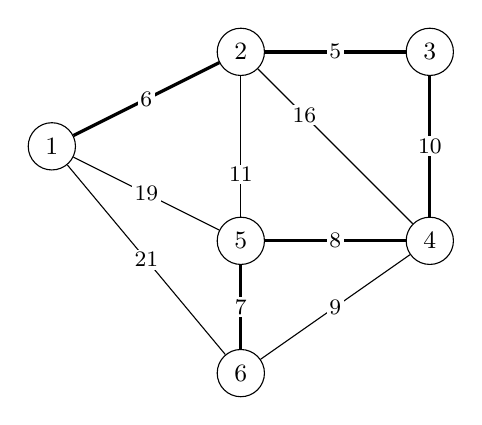
\begin{tikzpicture}[x=1.2cm,y=1.2cm,v/.style={circle,draw,inner sep=0pt,minimum size=6mm,font=\small},
  w/.style={font=\footnotesize,fill=white,inner sep=1pt}]
\node[v] (1) at (0,1) {1};
\node[v] (2) at (2,2) {2};
\node[v] (3) at (4,2) {3};
\node[v] (4) at (4,0) {4};
\node[v] (5) at (2,0) {5};
\node[v] (6) at (2,-1.4) {6};
\draw[very thick] (1) -- node[w] {6} (2);
\draw (1) -- node[w] {19} (5);
\draw (1) -- node[w] {21} (6);
\draw[very thick] (2) -- node[w] {5} (3);
\draw (2) -- node[w,pos=0.3] {16} (4);
\draw (2) -- node[w,pos=0.7] {11} (5);
\draw[very thick] (3) -- node[w] {10} (4);
\draw[very thick] (4) -- node[w] {8} (5);
\draw (4) -- node[w] {9} (6);
\draw[very thick] (5) -- node[w] {7} (6);
\end{tikzpicture}
\end{center}
用 Kruskal 演算法（資結書第~24.2~節），邊依成本由小到大，兩端已連通就跳過：
\begin{center}
\small
\begin{tabular}{cccl}
\toprule
成本 & 邊 & 結果 & 加入後的連通塊（只列兩點以上的） \\
\midrule
5 & (2,3) & 加入 & $\{2,3\}$ \\
6 & (1,2) & 加入 & $\{1,2,3\}$ \\
7 & (5,6) & 加入 & $\{1,2,3\}$, $\{5,6\}$ \\
8 & (4,5) & 加入 & $\{1,2,3\}$, $\{4,5,6\}$ \\
9 & (4,6) & 跳過（4、6 已連通） & \\
10 & (3,4) & 加入 & $\{1,2,3,4,5,6\}$ \\
\bottomrule
\end{tabular}
\end{center}
加到第 $5 = 6 - 1$ 條邊就完成（上圖粗線）；其餘 $11, 16, 19, 21$ 的邊兩端都已連通。 最小成本
\[
5 + 6 + 7 + 8 + 10 = 36 .
\]
成本互不相同，最小生成樹唯一（資結書定理~24.4）。 用 Prim 從頂點 1 開始檢查：依序加入
$2$（成本 $6$）、$3$（$5$）、$4$（$10$）、$5$（$8$）、$6$（$7$），得到同一組邊，總和也是 $36$。
\end{pastsoln}
